\documentclass{ximera}
\title{Image Importing Basic Usage}

%\usepackage{svg}
\graphicspath{
{./}
{./missionPatch/}% Path from the ximera document file to the image file(s)
{../../testFiles/dtxTestFiles/image/missionPatch/}% Path from the xourse file to image file(s).
}% Only add a preamble file if it is actually necessary for the demo/test.
\begin{document}
\begin{abstract}
    Testing/demo for including images in documents.
\end{abstract}
\maketitle

{{\Huge \bfseries Last Updated: \today}} \\


\section{Basic Usage}
For more users, images should be located in the xmPictures folder which is automatically loaded.
However, you can also put images in a folder that is included using the \verb|\graphicspath| command.

Most common image formats are supported and work fine in the pdf, but due to how dynamic sizing in a browser works,
vector based graphic formats like SVG are preferable for online images, but require the ``svg'' package and using 
the command \verb|\includesvg| instead of \verb|\includegraphics| (currently commented out, pending result of issue on svg package resolution).

Default styling can be attained using the image environment, although it isn't necessary.

\section{Intended Outcome of Test}
Below should be a sequence of images - all of which are the ximera logo - but in different formats for demonstration. 
The first half are in image environments, the second half are not.

\section{Start of Test/Demo Area}


A TikZ image in an image environment:
\begin{image}
    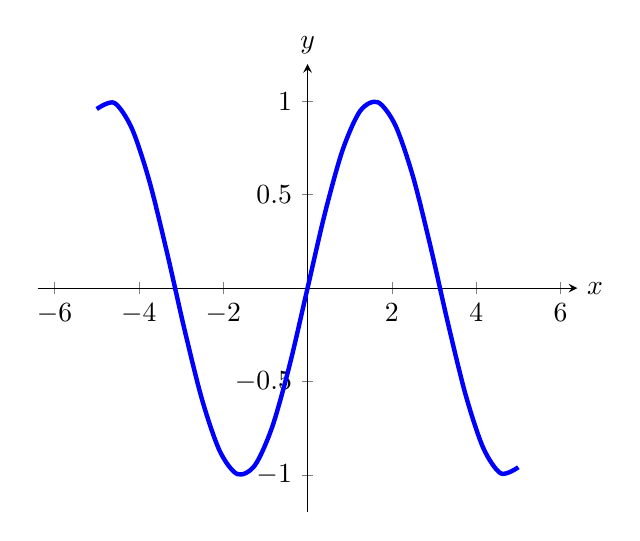
\begin{tikzpicture}
      \begin{axis}[
          xmin=-6.4,
          xmax=6.4,
          ymin=-1.2,
          ymax=1.2,
          axis lines=center,
          xlabel=$x$,
          ylabel=$y$,
          every axis y label/.style={at=(current axis.above
              origin),anchor=south},
          every axis x label/.style={at=(current axis.right of
              origin),anchor=west},
        ]
        \addplot [ultra thick, blue, smooth] {sin(deg(x))};
      \end{axis}
    \end{tikzpicture}
  \end{image}


%\begin{image}
%    svg format in an image environment:
%
%    \includesvg{missionPatch.svg}
%\end{image}
\hrulefill

A PNG in an image environment:
\begin{image}
    
\includegraphics{missionPatch.png}
\end{image}

\hrulefill

A PDF in an image environment:

\begin{image}
    
\includegraphics{missionPatch.pdf}
\end{image}

\hrulefill

A JPG format in an image environment:

\begin{image}
    
\includegraphics{missionPatch.jpg}
\end{image}

\hrulefill

\subsection{Repeat but in \texttt{center}}

\begin{center}
    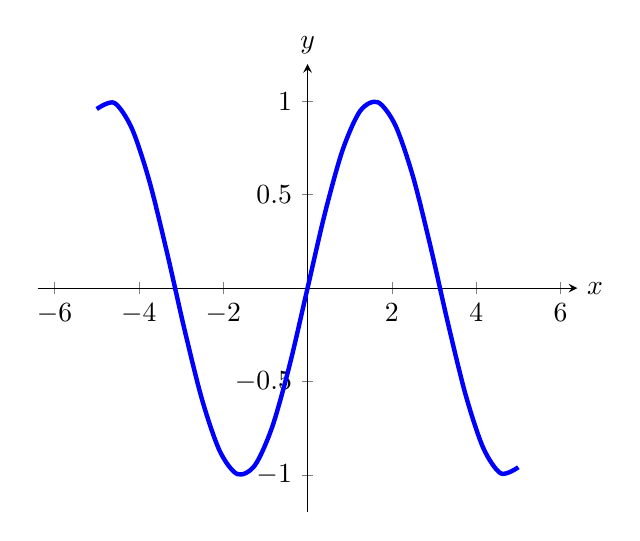
\begin{tikzpicture}
      \begin{axis}[
          xmin=-6.4,
          xmax=6.4,
          ymin=-1.2,
          ymax=1.2,
          axis lines=center,
          xlabel=$x$,
          ylabel=$y$,
          every axis y label/.style={at=(current axis.above
              origin),anchor=south},
          every axis x label/.style={at=(current axis.right of
              origin),anchor=west},
        ]
        \addplot [ultra thick, blue, smooth] {sin(deg(x))};
      \end{axis}
    \end{tikzpicture}
  \end{center}


%\begin{center}
%    svg format in an center environment:
%
%    \includesvg{missionPatch.svg}
%\end{center}
\hrulefill

A PNG in an center environment:
\begin{center}
    
\includegraphics{missionPatch.png}
\end{center}

\hrulefill

A PDF in an center environment:

\begin{center}
    
\includegraphics{missionPatch.pdf}
\end{center}

\hrulefill

A JPG format in an center environment:

\begin{center}
    
\includegraphics{missionPatch.jpg}
\end{center}

\end{document}
